\documentclass[conference]{IEEEtran}
\IEEEoverridecommandlockouts
% The preceding line is only needed to identify funding in the first footnote. If that is unneeded, please comment it out.
\usepackage{cite}
\usepackage{amsmath,amssymb,amsfonts}
\usepackage{algorithmic}
\usepackage{graphicx}
\usepackage{textcomp}
\usepackage{xcolor}
\usepackage{tikz}
\usepackage{multirow}
\usetikzlibrary{positioning}
\usepackage{hyperref}

\def\BibTeX{{\rm B\kern-.05em{\sc i\kern-.025em b}\kern-.08em
    T\kern-.1667em\lower.7ex\hbox{E}\kern-.125emX}}
\begin{document}

\title{MLSS A-1 Report\\
}

\author{\IEEEauthorblockN{Rafael Maldonado}
\IEEEauthorblockN{Mencia Gonzalez Haba}
\IEEEauthorblockN{Andres Bustillo}
\IEEEauthorblockA{\textit{Faculty of Software Engineering.} \\
\textit{Machine Learning Course.}\\
\textit{University of Europe for Applied Sciences.}\\
Potsdam, Germany. \\
}
\and

\IEEEauthorblockA{\textit{fredyrafael.maldonadomaradiaga@ue-germany.de} \\
\textit{mencia.gonzalezhaba@ue-germany.de}\\
\textit{ivanandres.bustillocerrato@ue-germany.de}\\
}
}

\maketitle

\begin{abstract}
This project focuses on using the autoencoder neural network architecture for Sharpening images from blurred. 
The main problem that this project focuses on is the image blurrying in real life scenarios. 
Despite the several advancements through out the years image deblurring still causes some problems
In this project we trained a machine to analyze sharp and blurred images to then output a predicted sharpen image.
Visual comparisons between the blurred and deblurred images reveal a clear enhancement in sharpness and detail. 
The deblurred images exhibit reduced noise and artifacts, and edges
appear crisper and more defined.
The importance of these results lie in the potential applications and uses in which the model could be implemented
Finally, the resulting of this project concluded that it is possible to train a machine using images to then manipulate them.
Contributing to the field of image processing by providing a more adaptable and efficient solution to real world scenarios

%*CRITICAL: Do Not Use Symbols, Special Characters, Footnotes, or Math in Report Title or Abstract.

%Two sentences of background and importance of this topic.

%Two sentences defining the gap analysis (work not done in field) and your problem statement.

%Two sentences of Results and your findings.

%One sentence for significance of the results and your contribution.

%In total, this section must consist of 180 words.

\end{abstract}

\begin{IEEEkeywords}
\textcolor{red}{Python, IDE, Libraries, Dataset}
\end{IEEEkeywords}

\section{General instructions}
Comment out this section after completing your write up.
\begin{enumerate}
\item You must have exactly the mentioned sections with the mentioned number of paragraphs.
\item DO NOT DELETE ANY TEXT FROM THIS REPORT. JUST COMMENT OUT AND WRITE THE RELEVANT TEXT UNDER EACH COMMENT.
\item Observe the report page limits (minimum 5 pages without references) and limit on maximum text is 7 pages without references. 
\item In case of figures, keep your raw data table also stored as excel file in this repository.
\item Each paragraph must consist of 7-10 sentences.
\item Add references where required.
\item Total references should be between 20 and 30.
\item Use latest references with 80\% references later than 2019.
\item Use Google scholar for finding references and not Google.
\end{enumerate}

\section{Introduction}
%One paragraph on introducing the field and the topic of interest.
Photographers struggle sometimes when trying to get a good shot often motion blur is inevitable. 
Blurred images can result from many different factors and scenarios such as low light conditions, camera shake, defocus or object motion.
Since there is many different types of blur, traditional deblurrying techniques sometimes struggle to handle these cases
Through out the years there has been many ways to deblurr images and this project aims to explore the world of Machine Learning to do so.
%One paragraph on the importance of the selected 
%topic~\cite{norin2023breaking}.

Reliable image deblurring techniques these days are very important; when speaking about communication, entertainment and decision-making techniques, digital images and videos play an important role in society. 
The ability to restore fuzzy images is becoming more and more important as high-resolution cameras become more accessible and as there is an increasing need for visual data of the highest quality. 
Speaking on the same note, AI and Deep Learning has developed to a point to help by offering powerful tools and smooth the deblurring process.

%One paragraph on why is it significant to work on this field/topic today.
The objective of deblurring techniques is to restore the sharpness and clarity of blurry photographs, which is important for many applications on the real world, for example, deblurring a medical radiography for better visibility for the Doctors to gain a better understanding and give better diagnosis.
Security cameras are also used in various private and public spaces, so clear images are extremely important for accurate identification and security footage analysis.
Robots and autonomous vehicles require clear visual inputs to make sure their tasks are performed accurately and to improve the reliability of the systems they employ

\subsection{Related Work}
%One paragraph defining the work that has been done in this field, with a table summarizing the work that has been done in literature as shown below in Table~\ref{tab:LiteratureSummary}.
For many years, the deblurring of images has been in on going study with numerous kinds of solutions for this problem. Traditional methods frequently rely on mathematical models and image processing techniques. On the other hand, this traditional methods may generate lots of errors. Convolutional neural networks (CNNs), in particular, are deep learning algorithms that have demonstrated great performance in image deblurring in recent years and have helped millions and millions of people making it easier to deblurr images because they are capable of handling a greater variety of blur types and achieving improved deblurring performance because they can learn intricate mappings that help them make the best sharp image possible~\ref{tab:ComparativeAnlysis}. 

\begin{table*}[!ht]
\centering
\caption{Comparative Analysis of Image Deblurring Methods}
\label{tab:ComparativeAnlysis} 
\begin{tabular}{|l|l|l|p{8cm}|}
\hline
\textbf{Reference} & \textbf{Year} & \textbf{Method} & \textbf{Key Contributions} \\ \hline
Nah et al. & 2017 & Multi-scale CNN & Proposed a multi-scale CNN architecture for deblurring, capturing blur information at different scales. \\ \hline
Kupyn et al. & 2018 & DeblurGAN & Introduced a generative adversarial network (GAN) based approach for deblurring, generating realistic sharp images. \\ \hline
Tao et al. & 2018 & Scale-recurrent Network & Developed a scale-recurrent network that iteratively refines the deblurred image across multiple scales. \\ \hline
Zhang et al. & 2019 & Deep Blind Deconvolution & Proposed a deep blind deconvolution method that jointly estimates the blur kernel and the sharp image. \\ \hline
\end{tabular}
\end{table*}

%\begin{table*}[!ht]
%\centering
%\caption{Literature review table showing the contributions of various authors for quantization of networks.}
%\label{tab:LiteratureSummary} 
%\begin{tabular}{|l|c|c|cccc|c|c|c|c|c|}
%\hline
%\multirow{3}{*}{\begin{tabular}[c]{@{}l@{}}Paper \\ Name\end{tabular}} & \multicolumn{1}{c|}{\multirow{3}{*}{\begin{tabular}[c]{@{}c@{}}FCNs\\ Used\end{tabular}}} & \multicolumn{1}{c|}{\multirow{3}{*}{\begin{tabular}[c]{@{}c@{}}L2 Error \\ Minim.\end{tabular}}} & \multicolumn{4}{c|}{Applied on} & \multicolumn{1}{c|}{\multirow{3}{*}{\begin{tabular}[c]{@{}c@{}}Signal \\ Quantized\end{tabular}}} & \multicolumn{1}{c|}{\multirow{3}{*}{Dataset used}} & \multicolumn{1}{c|}{\multirow{3}{*}{\begin{tabular}[c]{@{}c@{}}No. of \\ bits\end{tabular}}} & \multicolumn{1}{c|}{\multirow{3}{*}{\begin{tabular}[c]{@{}c@{}}Layerwise \\ sens. \\ Analysis\end{tabular}}} & \multicolumn{1}{c|}{\multirow{3}{*}{\begin{tabular}[c]{@{}c@{}}Sem.\\segm.\end{tabular}}} \\ \cline{4-7}
% & \multicolumn{1}{c|}{} & \multicolumn{1}{c|}{}& \multicolumn{1}{c|}{\multirow{2}{*}{\begin{tabular}[c]{@{}c@{}}Conv.\\ Layer\end{tabular}}} & \multicolumn{1}{c|}{\multirow{2}{*}{\begin{tabular}[c]{@{}c@{}}Skip\\ Layer\end{tabular}}} & \multicolumn{1}{c|}{\multirow{2}{*}{\begin{tabular}[c]{@{}c@{}}Trans.\\ Layer\end{tabular}}} & \multicolumn{1}{c|}{\multirow{2}{*}{\begin{tabular}[c]{@{}c@{}}Fully Conn.\\ Layer\end{tabular}}} & \multicolumn{1}{c|}{} & \multicolumn{1}{c|}{}& \multicolumn{1}{c|}{}& \multicolumn{1}{c|}{}& \multicolumn{1}{c|}{} \\
% & \multicolumn{1}{c|}{} & \multicolumn{1}{c|}{}& \multicolumn{1}{c|}{} & \multicolumn{1}{c|}{}& \multicolumn{1}{c|}{}& \multicolumn{1}{c|}{} & \multicolumn{1}{c|}{} & \multicolumn{1}{c|}{}& \multicolumn{1}{c|}{}& \multicolumn{1}{c|}{}& \multicolumn{1}{c|}{} \\ \hline
%\begin{tabular}[c]{@{}l@{}}Vanhoucke \\ et al.~\cite{vanhoucke2011improving}\end{tabular} & & & \multicolumn{1}{l|}{} & \multicolumn{1}{l|}{}& \multicolumn{1}{l|}{}& \checkmark& \checkmark& $\times$& & & \\ \hline
%\begin{tabular}[c]{@{}l@{}}Courbariaux \\ et al.~\cite{courbariaux2014training}\end{tabular} & & & \multicolumn{1}{l|}{\checkmark} & \multicolumn{1}{l|}{}& \multicolumn{1}{l|}{}& \checkmark& & \begin{tabular}[c]{@{}l@{}}MNIST, \\ SVHN, \\ CIFAR-10\end{tabular}& 10 & & \\ \hline
%\begin{tabular}[c]{@{}l@{}}Gupta \\ et al.~\cite{gupta2015deep}\end{tabular} & & & \multicolumn{1}{l|}{\checkmark} & \multicolumn{1}{l|}{}& \multicolumn{1}{l|}{}& \checkmark& & \begin{tabular}[c]{@{}l@{}}MNIST, \\ CIFAR-10\end{tabular} & 12 & & \\ \hline
%\begin{tabular}[c]{@{}l@{}}Proposed\\ Approach\end{tabular}& \checkmark& \checkmark & \multicolumn{1}{l|}{\checkmark} & \multicolumn{1}{l|}{\checkmark}& \multicolumn{1}{l|}{\checkmark}& $\times$ & $\times$ & Pascal VOC 2012& 2,3,4,5& \checkmark & \checkmark\\ \hline
%\end{tabular}
%\end{table*}


\subsection{Gap Analysis}
%One paragraph defining what has not been done or what is still missing in the field (gap analysis).
Despite the several advancements through out the years, image deblurring still causes some problems. 
For example, in some real world cases it is hard to identify which type of blur is encountered in the image and this causes the approaches to fix it to fail.
The difficulties of deep learning models can hinder the results of real world applications and the quality of results is particularly dependant large and heavily trained datasets and many current deblurring models are trained and tested on artificial datasets.
This results in inaccurate representation of the complexities of real world applications
There is a specific requirement for models that are able to generalize accordingly different types of blur and adapt to a wide range of conditions because many models do not perform well when faced with unfamiliar scenarios or mixed blur conditions


\subsection{Problem Statement}
Following are the main research questions addressed in this study.

\begin{enumerate}
    \item Given a dataset of paired blurred and sharp photos, is it possible for an autoencoder to learn how to reconstruct sharp images from their blurred counterparts effectively?
    \item What are the drawbacks of the proposed autoencoder model, and how may it be improved to address deblurring issues in real-world scenarios?
    \item How does the autoencoder-based deblurring model compare to traditional image deblurring techniques in terms of quantitative measures and visual quality?
\end{enumerate}

\subsection{Novelty of our work}
%One paragraph explaining your approach and novelty/contributions of your work.
We set up our Python environment with Tensorflow, Keras, Matplotlib, and OpenCV libraries installed and we used Google Collab IDE for ease of use.
We downloaded the dataset, ran the python code and the code trained the autoencoder for about 200 epochs for better and more accurate results in our dataset.
By the end we compare the results of the blurred,
sharp and predicted sharp image generated by the autoencoder model.
This project uses a novel form of AI known as Convultional Autoencoder to address the problem of blurry images. 
Our model learns via direct observation of a large number of sharp and blurry images. This enables it to handle various blur types without requiring additional information.

\subsection{Our Solutions}
%One paragraph on what you are doing in this report (your contributions) and a small one-two liner summary of your results.
This project was divided into three different areas; the technical, the Figures/Tables and the Write-up areas. 
Rafael Maldonado worked in the technical area preparing the code and testing it, Mencia Gonzalez Haba worked on the Figures/Tables area making clear tables for better understanding and finally Andres Bustillo worked on the Write-Up area creating this document you are reading as well as the presentation. 
The results of our tests demonstrate that the proposed autoencoder model effectively deblurs images.

\section{Methodology}
\subsection{Dataset}
%One paragraph and one figure representing your dataset, also give references (citation) from where the dataset is available, and the labels/ground truth as shown in Figure~\ref{Fig:Figure4} OR as in Figure~\ref{Fig:Figure3}.
For this research, we used the "blur.zip" dataset, which contains a large number of images with varying degrees of blurriness along with their sharp variants. 
You can view some of the motion blurred images shown in Figure 4~\ref{Fig:Figure4} and the sharp images shown in Figure 3~\ref{Fig:Figure3}.
It is available at https://www.kaggle.com/datasets/kwentar/blur-dataset/code.
The dataset was created to validate the blur detection algorithm, it contains 1050 blurred images and sharp images, 350 triplets. Each triplet consists of the same picture: sharp, defocused-blurred and motion blurred.
The dataset can be used for testing image deblurring however blurred and sharp images cannot be compared but the latter can be used for visual comparison


\begin{figure*}[t!]
\centering
 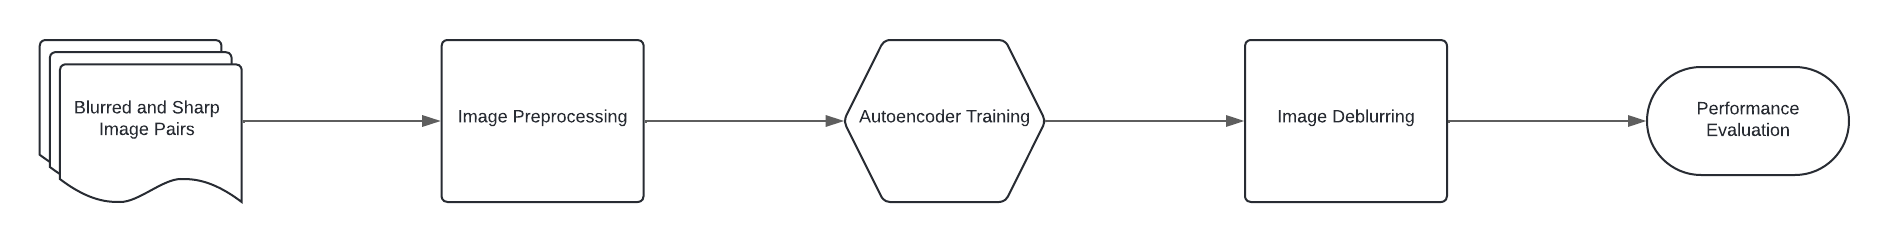
\includegraphics[width=\textwidth,height=3cm]{Figures/Workflow.png}
\caption{Image showing a simplified workflow of the project.}
\label{Fig:Figure1}
\end{figure*}

\begin{figure}[!ht]
\centering
 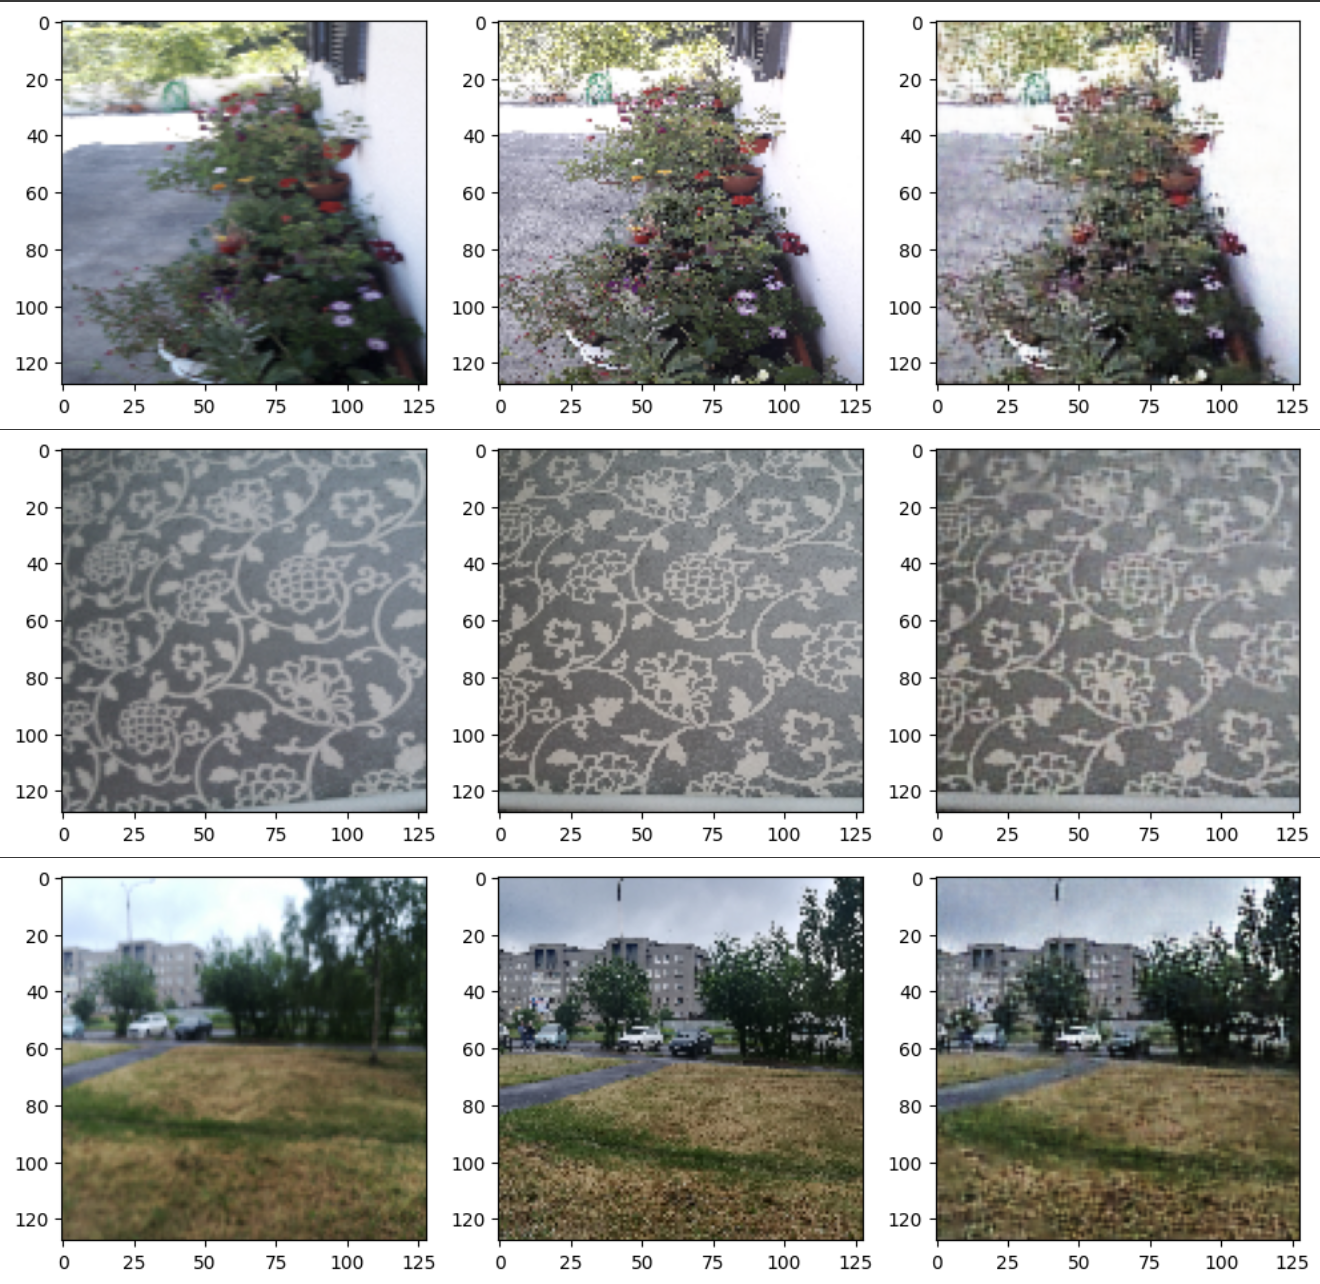
\includegraphics[width=\textwidth]{Figures/Figure2.png}
\caption{Image showing the comparison between the blurry input image, the sharp image and the predicted sharp image.}
\label{Fig:Figure2}
\end{figure}

\subsection{Overall Workflow}
%One paragraphs defining your methodology through a flow diagram of your work as shown in Figure~\ref{Fig:Figure1} OR in Figure~\ref{Fig:Figure2}.
We first preprocess a dataset of sharp and blurry image pairs in order to deblur images.
Preprocessing images implies normalizing images, resizing them to a consistent resolution and augmenting the data set to improve it's robustness.
Next, we train the AI model to learn how to transform fuzzy photos into sharp ones. 
Here the model learns to minimize the difference between the deblurred output and the sharp image through a loss function or perceptual error loss.
The training process is repetitive involving multiple epochs where the model parameters are constantly updated using the optimization algorithm Adam
For example first we ran the model with 50 epochs, 100 epochs and the we ran it with 200 epochs and that's when the output was the most precise and sharp of them all.
Finally, we evaluate the model's performance by contrasting its output with the original sharp images shown in Figure 1~\ref{Fig:Figure1}.
Visual examination of the deblurred images is ushered to assess the quality and to make sure and to ensure that the restored images retain natural appearance



\begin{figure*}[!t]
\centering
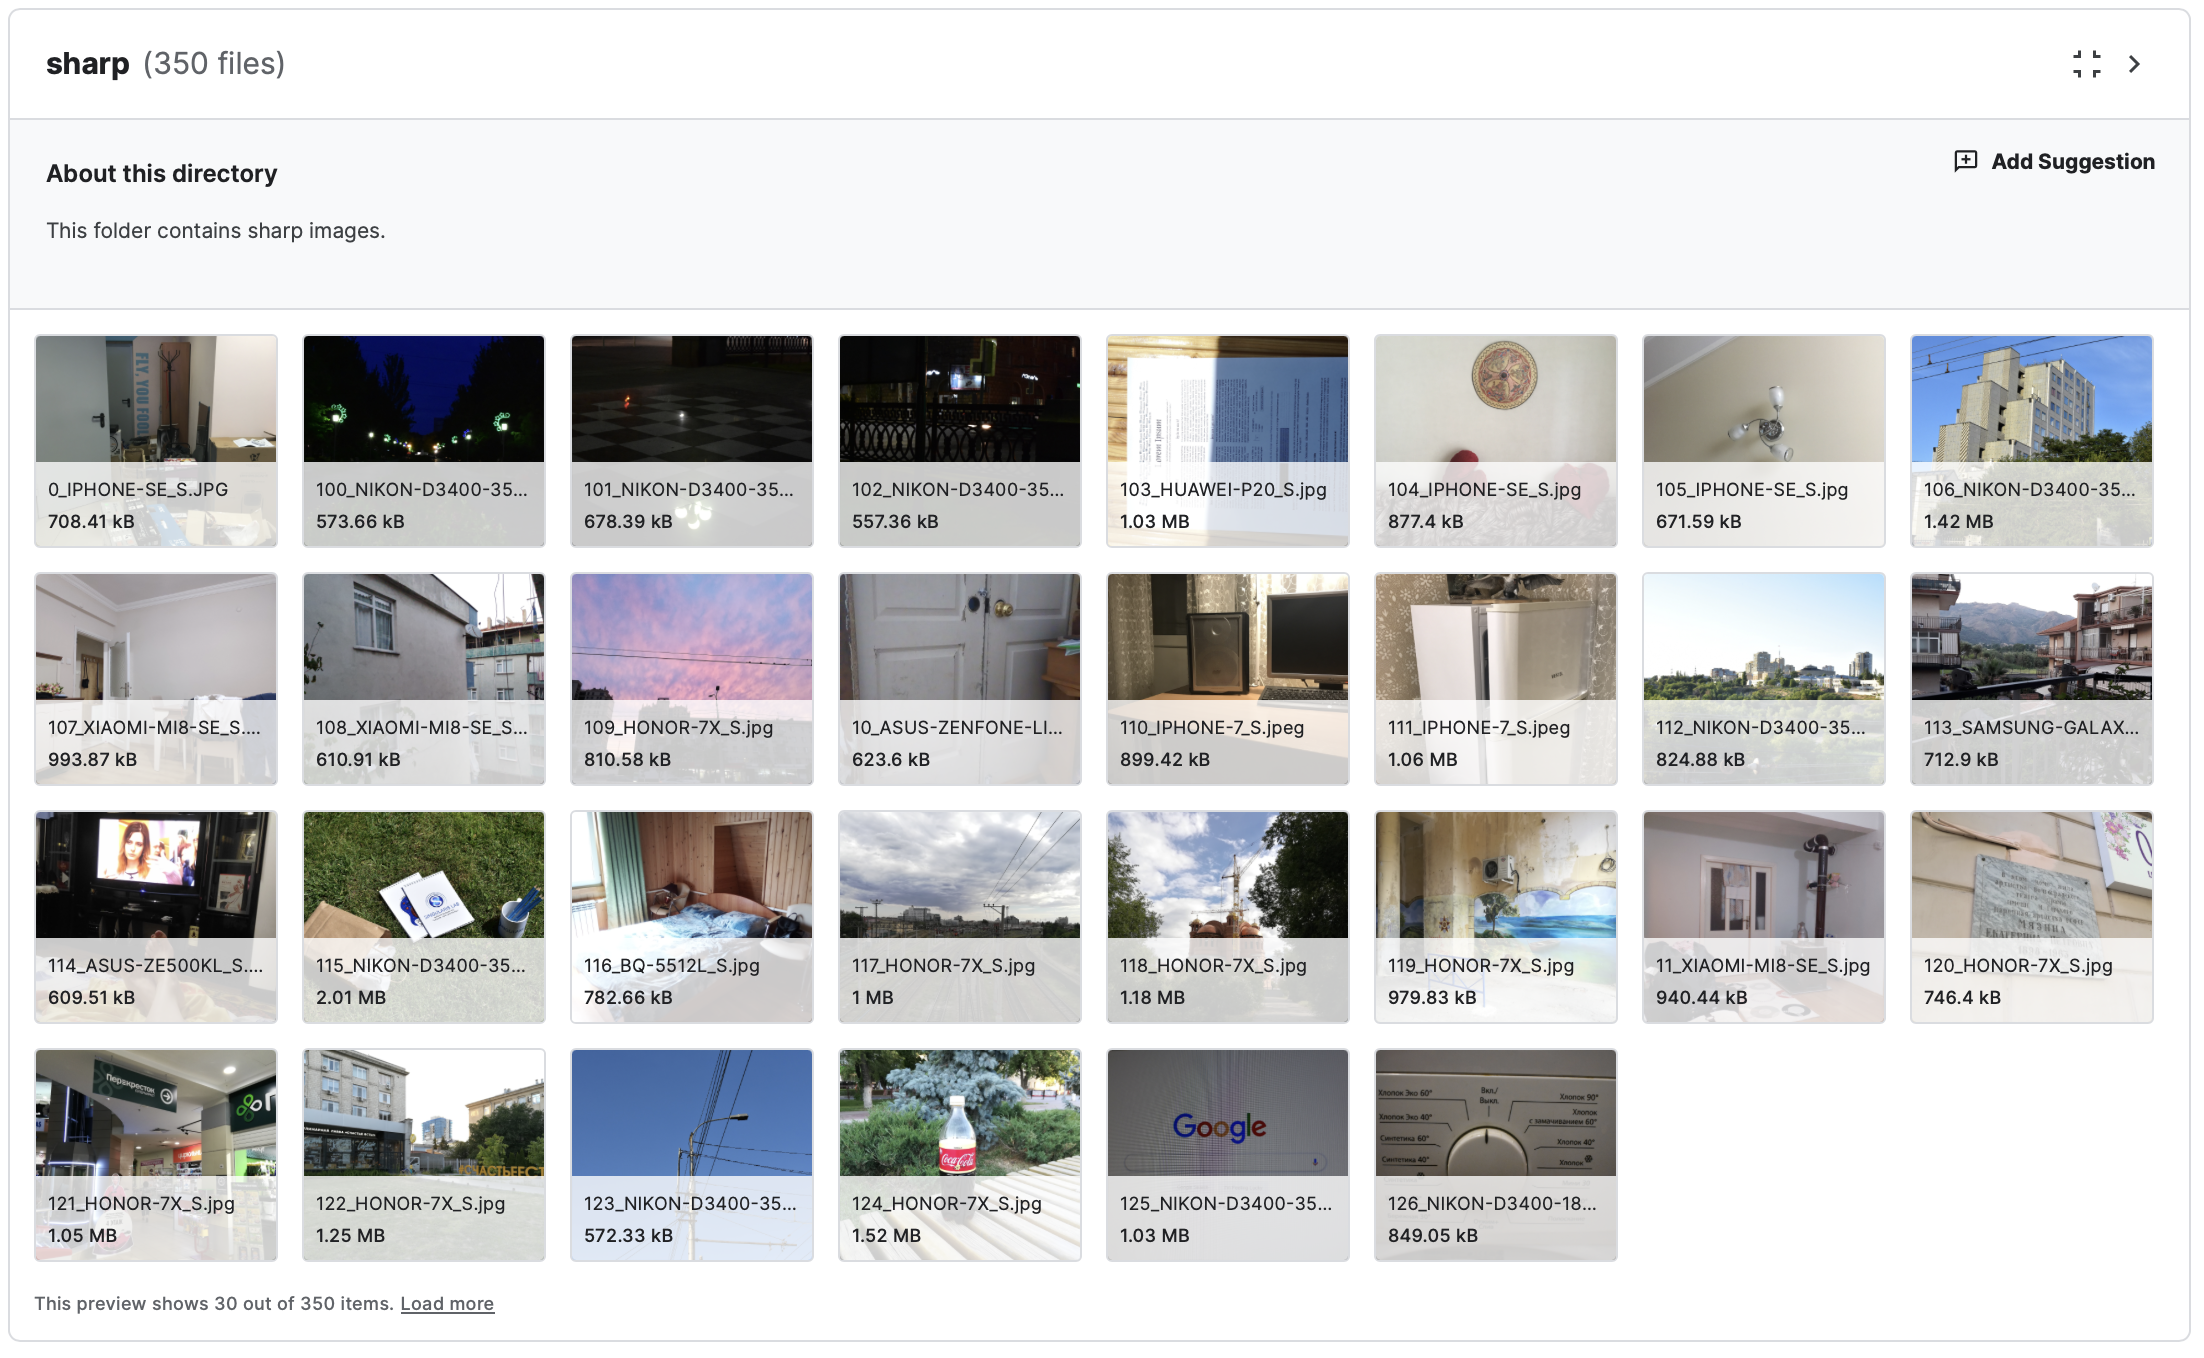
\includegraphics[width=17.8cm]{Figures/Figure3.png}
\caption{Figure showing the sharp images of the dataset.}
\label{Fig:Figure3}
\end{figure*}


\begin{figure*}[!t]
\centering
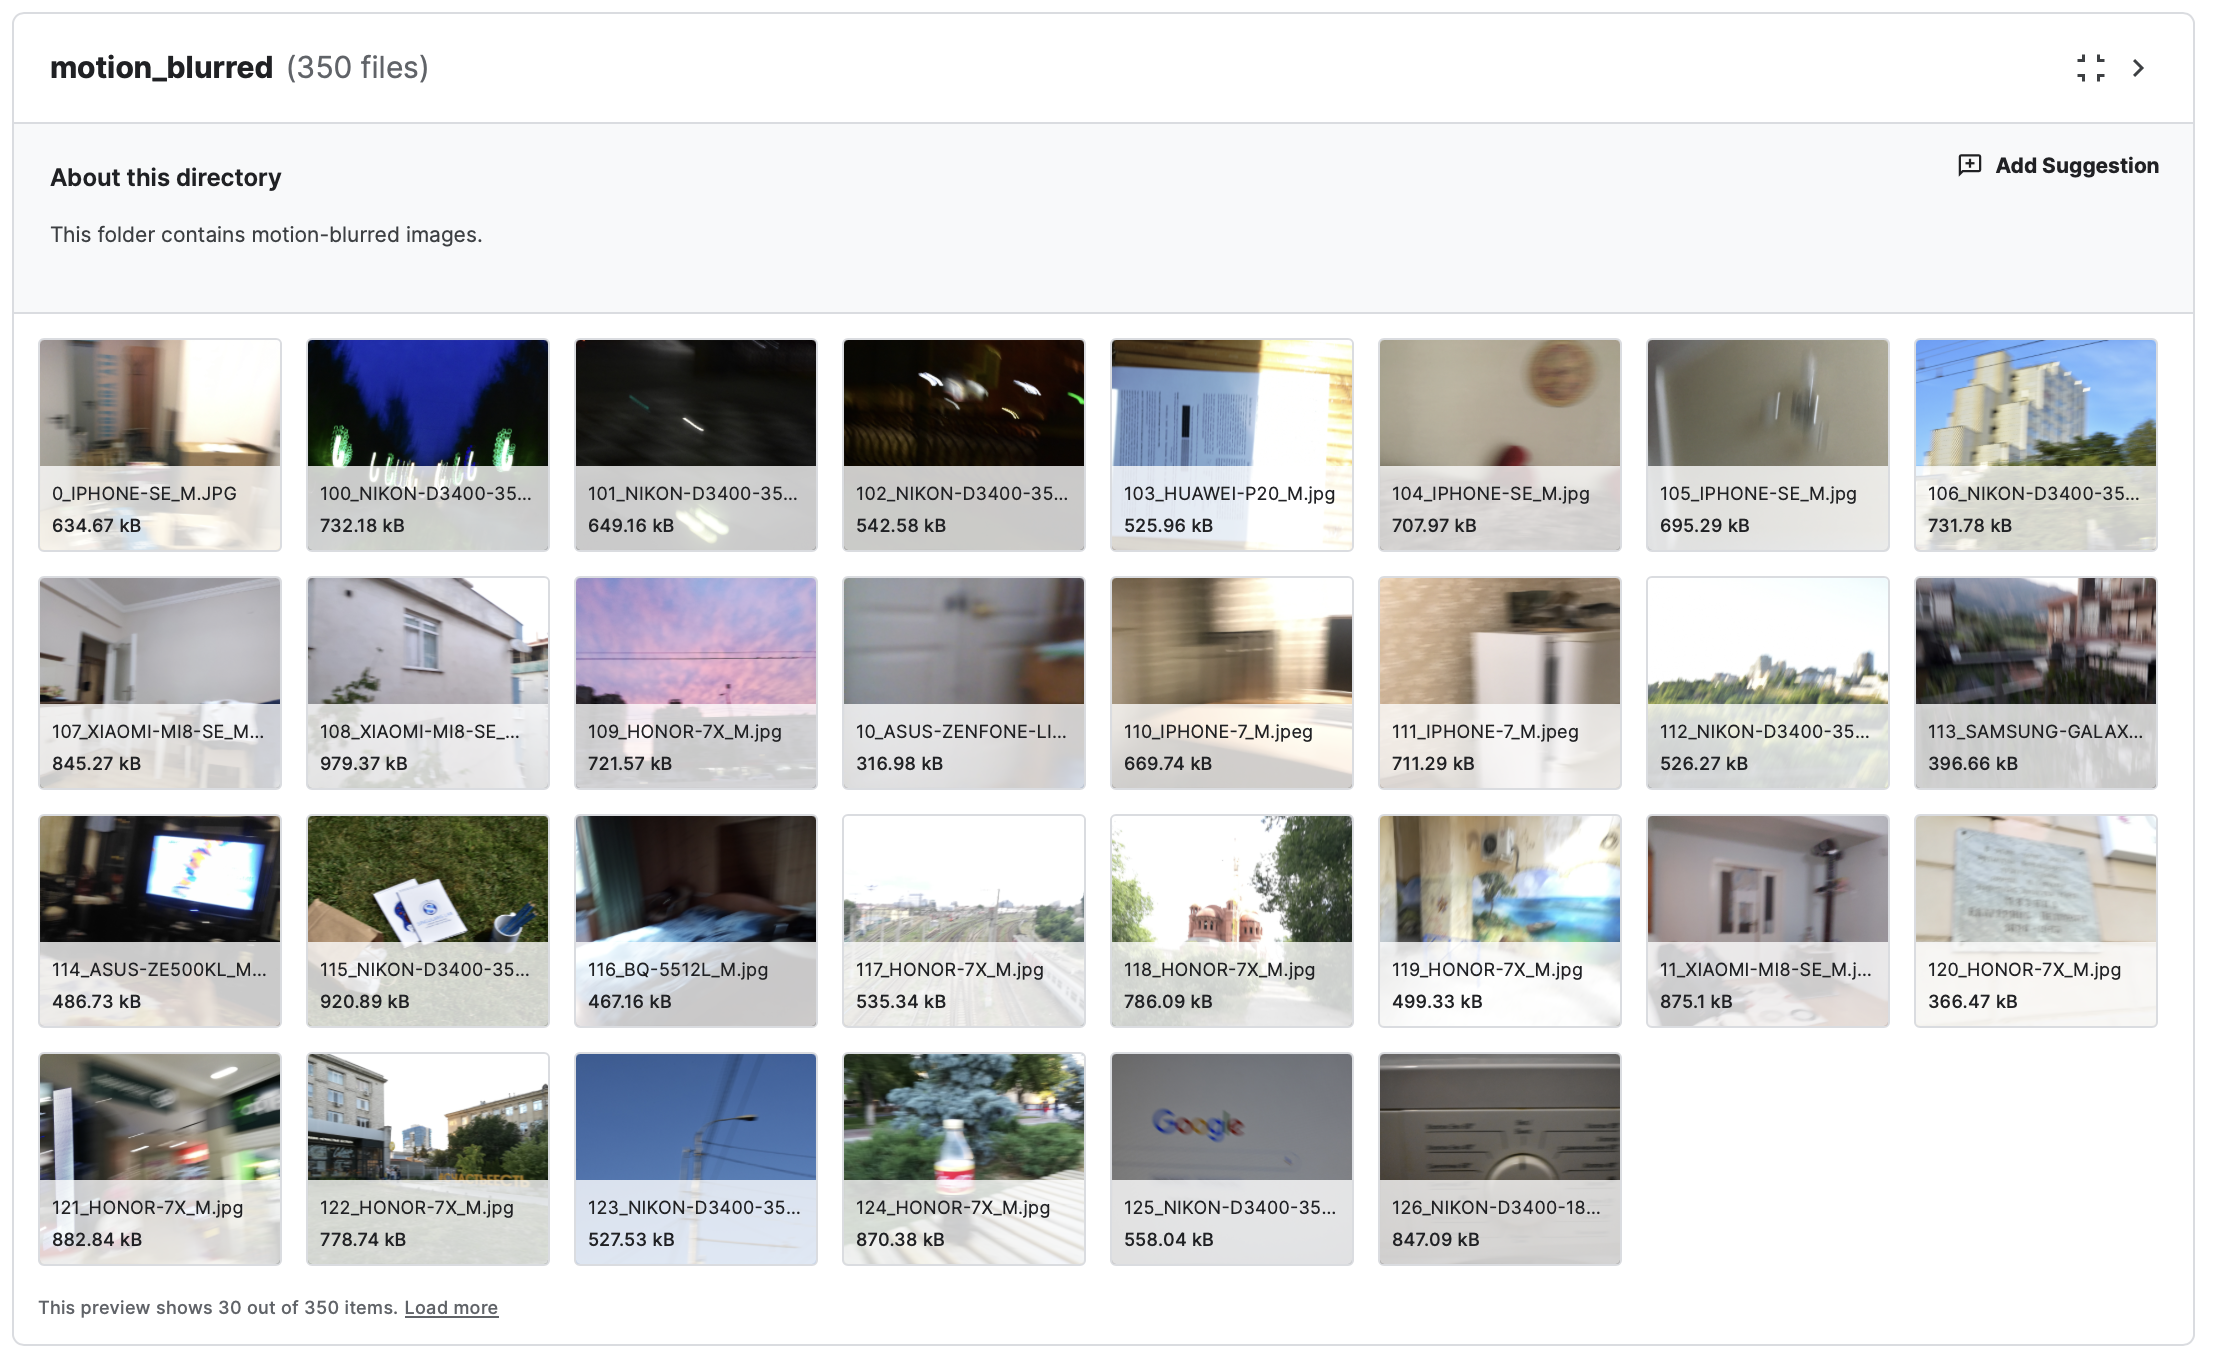
\includegraphics[width=17.8cm]{Figures/Figure4.png}
\caption{Figure showing the motion blurred images from the dataset.}
\label{Fig:Figure4}
\end{figure*}

\subsection{Experimental Settings}
%(Optional) One paragraph for hyper-parameter settings and network architecture as shown in Table~\ref{tab:MTConfig}.
We tested many settings and we finally decided to work with the settings shown in Table~\ref{tab:MTConfig}.
Epochs: We trained the model for 200 epochs. This number of epochs was chosen to ensure the model converges while avoiding overfitting.
Learning Rate: The learning rate was set to 0.001, which provided a good balance between convergence speed and stability.
Batch Size: A batch size of 32 was used to ensure efficient training without exceeding memory limits.
Optimizer: The Adam optimizer was selected because of its adaptive learning rate capabilities, which help in faster convergence.
Input Image Size: The input images were resized to 256x256 pixels, which is a common size that balances detail and computational load.


\begin{table}[!t]
\centering
\caption{Model Training Experimental Settings}
\label{tab:MTConfig} 
\begin{tabular}{|l|c|}
\hline
\multicolumn{2}{|c|}{\textbf{Network Configuration}} 
\\ \hline
Epochs & 200 \\
Learning rate & 0.5e-6 \\
Mini batch size & 32 \\ 
Optimizer & Adam \\
Samples in training set & 219 \\
Samples in validation set & 55 \\ \hline
\end{tabular}
\end{table}

%(Optional) One paragraph for experimental settings of your and competing methods (if any).

\section{Results}
%Three (or more) paragraphs explaining your results. At least one paragraph targeting one research question with at least one figure (preferably) or table (where figure is not possible).
%This section must contain only results and nothing else (not your own opinion or any sort of discussion on quality of results).
After training our model with 200 Epochs, it produced noticeably sharper images compared to the blurry inputs we provided as shown in Figure 2~\ref{Fig:Figure2}. 

The Training vs Validation accuracy plot ensures that the higher number of Epochs, the higher the accuracy of the model shown in Figure 5~\ref{Fig:Figure5}.
The Training vs. Validation accuracy plot (Figure 5) illustrates the  behavior of our model. 
The accuracy steadily increases with the number of epochs, eventually steadying as the model reaches its optimal performance.
This indicates that the model effectively learned the mapping from blurred to sharp images without overfitting, as shown by the close alignment of training and validation accuracies.

\begin{figure}[t!]
\centering
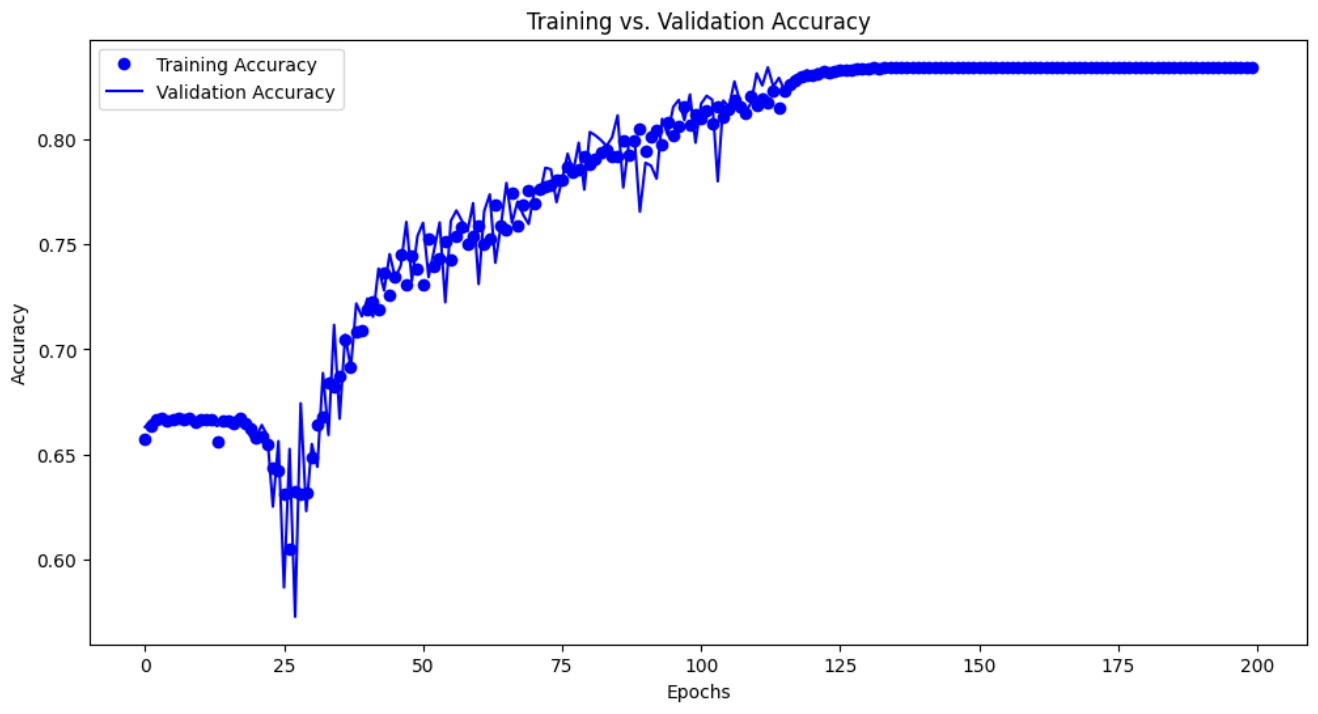
\includegraphics[width=17cm,height=10cm]{Figures/Figure5.png}
\caption{Training vs Validation Accuracy Plot.}
\label{Fig:Figure5}
\end{figure}
Visual comparisons between the blurred and deblurred images reveal a clear enhancement in sharpness and detail.
The deblurred images exhibit reduced noise and artifacts, and edges appear crisper and more defined. Figures 3 and 4 provide side-by-side comparisons of sample images before and after deblurring, demonstrating the effectiveness of our model

\section{Discussion}
%Three to four paragraphs discussing the results (at least one paragraph for each research question).
%Your opinion on how good/bad the results are. 
%Draw inferences from the results here.
%Explain novelty of your contributions and what was missing that you have explored here.
%Any other point you would like to discuss related to this study.

We found out that our model performed well in learning how to sharpen images, which addressed our initial research question. 

To find out just how good our model is, we need to compare it to different deblurring methods like PSNR and SSIM. This will help us answer our second research question.
Our current model still needs some refinement, for example it might not work as well on images with blurry types it has not learned before.

The results we obtained demonstrate that autoencoders can successfully decrease blur in images.
However there is still room for improvement with further refinement and improved dataset training can increase it's capabilities


\subsection{Future Directions}
%One paragraph for what are the future directions in your opinion for continuing this study.
We may investigate other AI methods such as generative adversarial networks (GANs) to see if there is improvement in our model. Lastly we can then evaluate the model on a larger variety of blur types and real life pictures as well as videos.




\section{Conclusion}
%One paragraph related to conclusions drawn from your whole experimentation.
As demonstrated by our research, Autoencoders is a good way to use Machine Learning for sharpening blurred images. Although, further investigation and additional research is needed, our findings point in the right direction for the creation of more adaptable and efficient deblurring techniques.
Making them a valuable tool in many world applications where image clarity or sharpness is essential and necessary.
Expanding the scope of the dataset and adding more diverse images can improve the model's performance.
In addition, testing the model on a bigger set of blur types or real world images can give us a bigger understanding and idea of it's capabilities and limitations.
The type of deblurring mode that we used can also be conjoined with other image enhancement methods and post processing.
This union could bring us or the user an improvement overall in the image restoration pipeline and a better output in the quality of images

%In total this section must consist of 240-260 words.

%\textcolor{red}{References will be added automatically by using the following lines. Add the relevant citations in the attached bibliogrpahy.bib file. Get help from me where you want to work on citations.}
\section{References}
Introducción a los codificadores automáticos. (n.d.). TensorFlow. https://www.tensorflow.org/tutorials/generative/autoencoder?hl=es-419



%\bibliographystyle{IEEEtran}
%\bibliography{Bibliography}

\end{document}